\section{Experiment and Results}
\vspace{-1.5mm}

\begin{table*}[!t]
\centering
\footnotesize
\caption{\textbf{Efficiency metrics for LLaMA-2-13B.} Left to right: 
XDomainBench (averaged across Selected/OOD/Cross); CommonsenseQA; Natural Questions; ARC.
Columns: Type (Dense/Light/Heavy), Ret. (head retention ratio), Mem. (memory in GB), Spd. (speedup).}
\setlength{\tabcolsep}{2pt}
\renewcommand{\arraystretch}{1.05}
\vspace{-2mm}
\begin{tabular}{@{}c@{\hspace{0.3em}}c@{\hspace{0.3em}}c@{\hspace{0.3em}}c@{}}
\begin{tabular}{l c c c}
\toprule
\textbf{Type} & \textbf{Ret.} & \textbf{Mem.} & \textbf{Spd.} \\
\midrule
Dense & --- & 13.0 & 1.00 \\
Light & 80.7\% & \underline{12.1} & \underline{1.26} \\
Heavy & 72.2\% & \underline{11.7} & \underline{1.24} \\
\bottomrule
\end{tabular} &
\begin{tabular}{l c c c}
\toprule
\textbf{Type} & \textbf{Ret.} & \textbf{Mem.} & \textbf{Spd.} \\
\midrule
Dense & --- & 13.0 & 1.00 \\
Light & 89.9\% & \underline{12.7} & \underline{1.08} \\
Heavy & 69.4\% & \underline{12.0} & \underline{1.09} \\
\bottomrule
\end{tabular} &
\begin{tabular}{l c c c}
\toprule
\textbf{Type} & \textbf{Ret.} & \textbf{Mem.} & \textbf{Spd.} \\
\midrule
Dense & --- & 13.0 & 1.00 \\
Light & 81.5\% & \underline{12.4} & \underline{1.08} \\
Heavy & 69.5\% & \underline{12.0} & 0.97 \\
\bottomrule
\end{tabular} &
\begin{tabular}{l c c c}
\toprule
\textbf{Type} & \textbf{Ret.} & \textbf{Mem.} & \textbf{Spd.} \\
\midrule
Dense & --- & 13.0 & 1.00 \\
Light & 80.2\% & \underline{12.4} & \underline{2.21} \\
Heavy & 68.3\% & \underline{12.0} & \underline{1.76} \\
\bottomrule
\end{tabular} \\     
\end{tabular}
% \vspace{-1mm}
\label{tab:efficiency_main}
\end{table*}

\begin{figure*}[!t]
  \centering
  \begin{subfigure}[b]{0.31\textwidth}
    \centering
    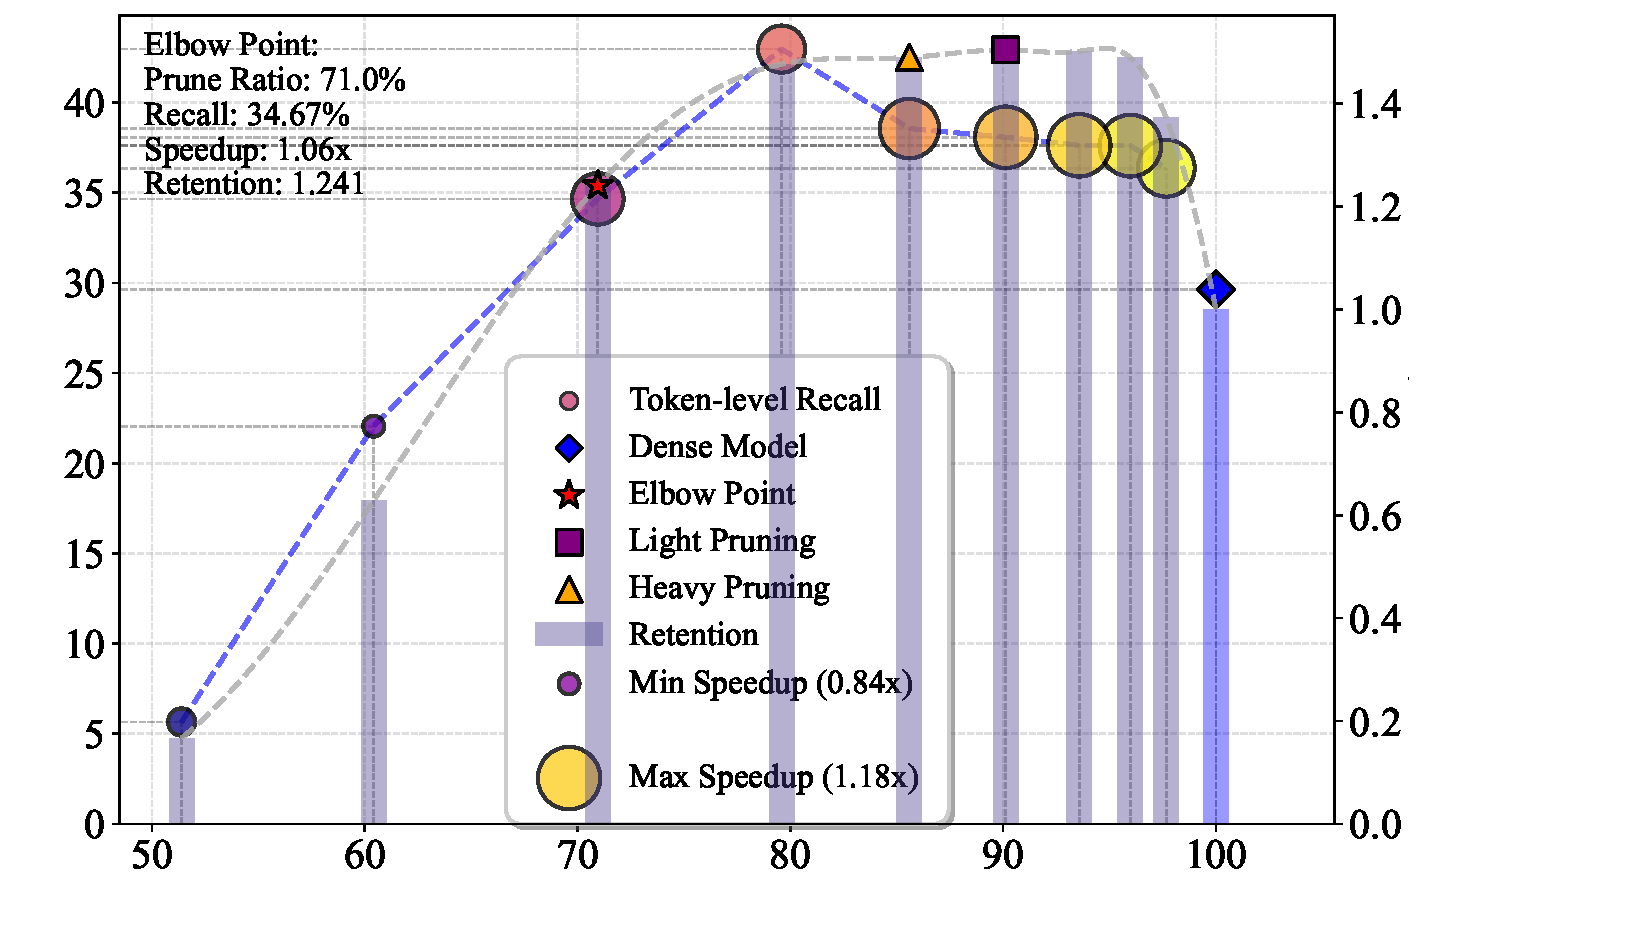
\includegraphics[width=\textwidth]{figs/tradeoff2/pruning_tradeoff_LLaMA_13B_single_main.pdf}
    \label{fig:pruning_tradeoff_single}
  \end{subfigure}
  \begin{subfigure}[b]{0.31\textwidth}
    \centering
    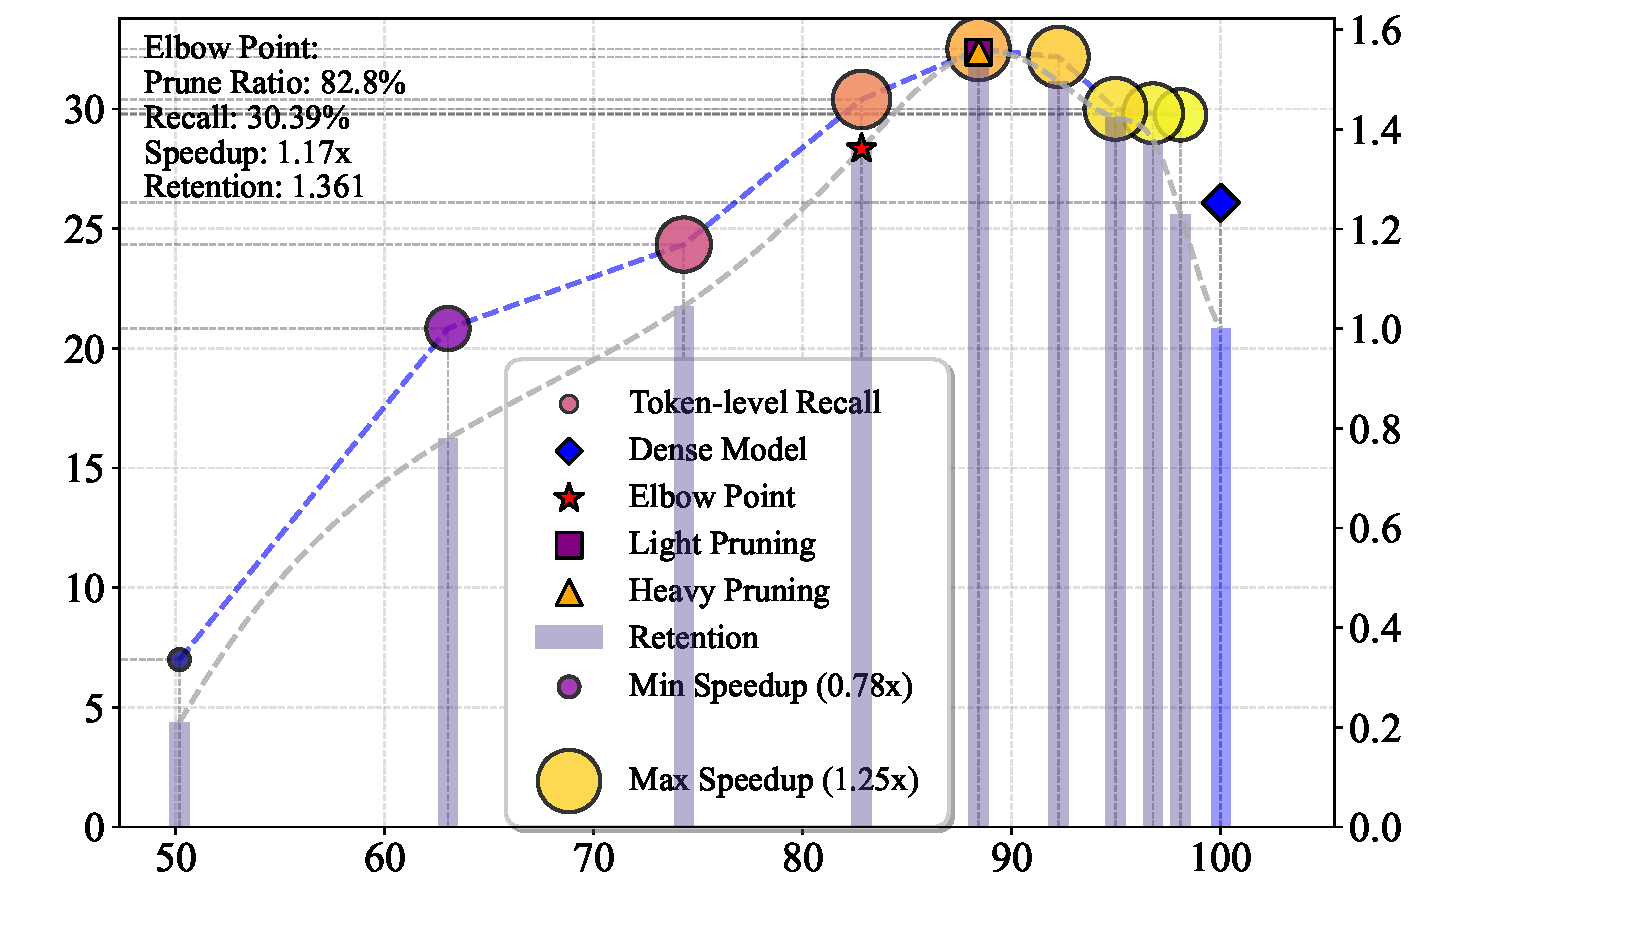
\includegraphics[width=\textwidth]{figs/tradeoff2/pruning_tradeoff_LLaMA_13B_ood_main.pdf}
    \label{fig:pruning_tradeoff_ood}
  \end{subfigure}
  \begin{subfigure}[b]{0.36\textwidth}
    \centering
    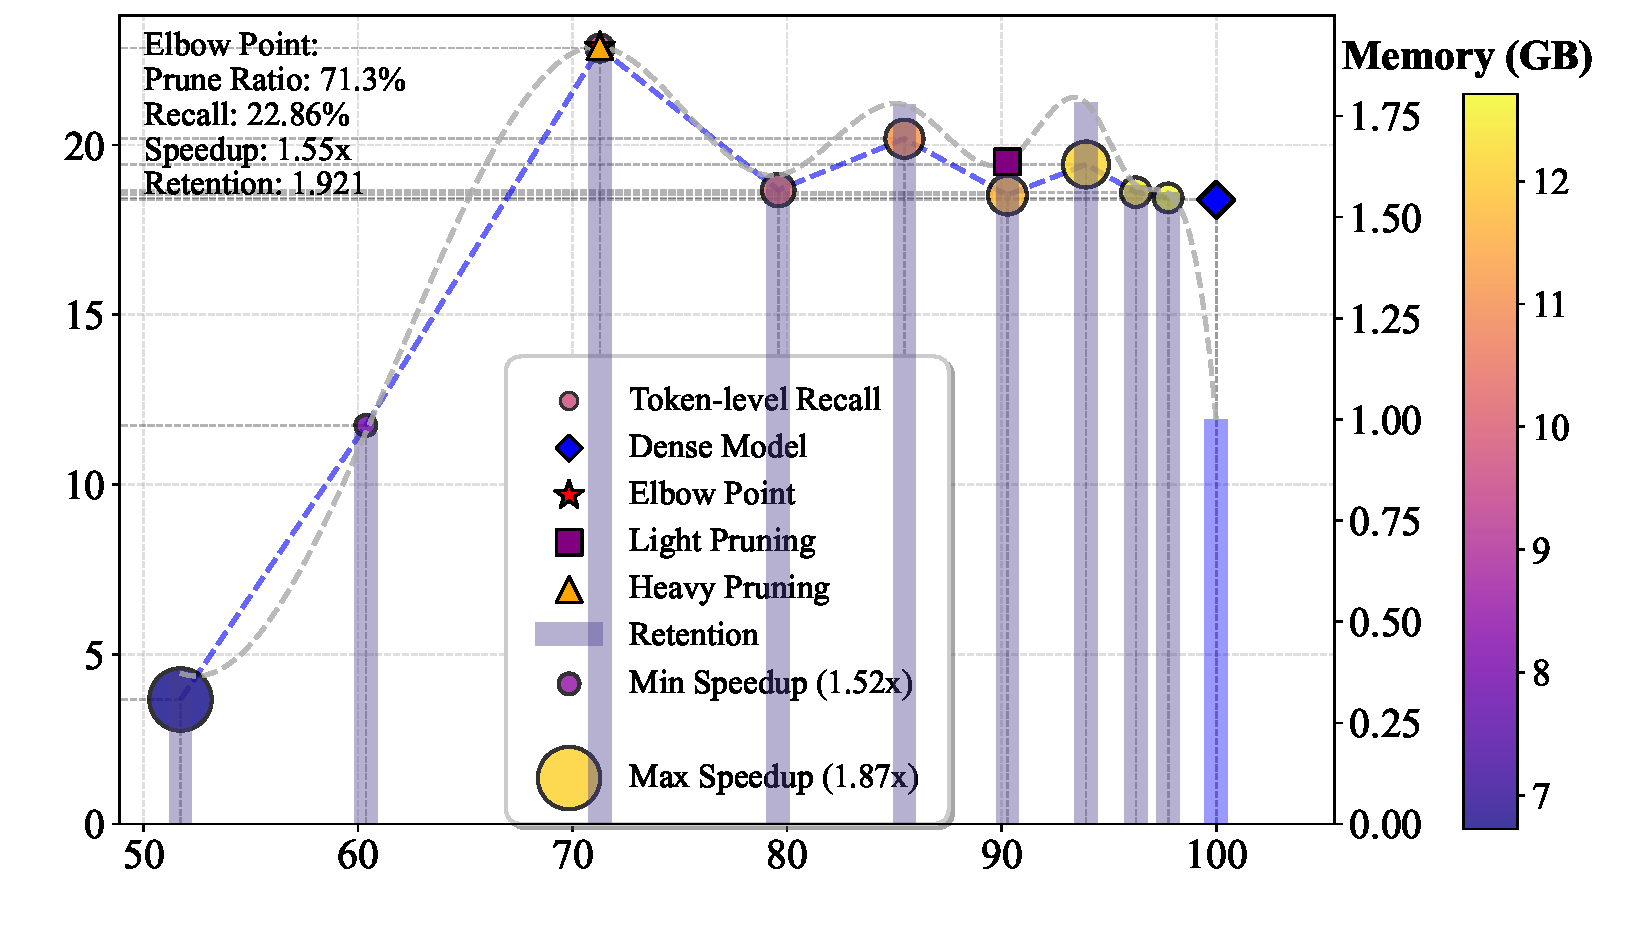
\includegraphics[width=\textwidth]{figs/tradeoff2/pruning_tradeoff_LLaMA_13B_cross_main.pdf}
    \label{fig:pruning_tradeoff_cross}
  \end{subfigure}
  \vspace{-4mm}
  \caption{\textbf{Pruning ratio vs Performance for LLaMA-2-13B.} 
  X-axis: Head retention (\%); Left/right Y-axis: Recall/ Retention.
  From left to right: selected, out of, and cross domain.
  Extended trade-off curves for all models and datasets are provided in Figures~\ref{fig:pruning_tradeoff_llama13b} and~\ref{fig:pruning_tradeoff_qwen7b}.}
  \vspace{-1mm}
  \label{fig:pruning_tradeoff}
\end{figure*}


% \vspace{-0.5em}
\label{sec:experiments}
\subsection{Experimental Setup}
\vspace{-1.5mm}
Our evaluation is designed to rigorously assess the efficacy and robustness of \emph{SubspacePath Pruner}, especially under cross-domain and cross-dataset generalization with budget constraints, and explore the trade-offs between pruning ratio, inference efficiency, and task performance. 

\textbf{Models.}  
We select four representative general-purpose LLM bases with distinct scales: \textbf{\textit{(i)}} \textbf{LLaMA‑2-13B-chat} and \textbf{\textit{(ii)}} \textbf{LLaMA-3.1-8B-Instruct} of Transformer-based pretrained language models~\cite{touvron2023llama}. \textbf{\textit{(iii)}} \textbf{Qwen2.5‑14B-Instruct} and \textbf{\textit{(iv)}} \textbf{Qwen2.5‑7B-Instruct} including dense decoder models at multiple parameter scales~\cite{yang2024qwen25}. Model versions, metrics, and configuration details are provided in Appendix~\ref{app:model_protocol}.

\textbf{Datasets.}  
We evaluate on XDomainBench split into selected-domain, out-of-domain, and cross-domain sets~\cite{gong2026xdomainbench}, CommonsenseQA~\cite{talmor2019commonsenseqa}, Natural Questions~\cite{kwiatkowski2019natural}, and ARC~\cite{clark2018arc}. We conduct \emph{offline} preparation only on a subset of the selected-domain portion of XDomainBench, with \emph{online} inference and testing performed on the remaining portions and other datasets. Dataset details, preprocessing procedures, and statistics are in Appendix~\ref{app:dataset_setup}.

\textbf{Baseline Methods.}  
We compare \textsc{SubspacePath Pruner} with several representative inference‑time training‑free compression methods under the same pruning ratios, with unpruned dense models. For unstructured methods, we selected 
% SparseGPT~\cite{frantar2023sparsegpt} and 
DaSS~\cite{guo2024dass}. For structured methods, we selected Wanda~\cite{sun2023wanda} and LLM-Pruner~\cite{llmpruner2023}.
% , and FASP~\cite{hu2025fasp}. 
For activation-/probe-guided methods, we selected RIA~\cite{zhang2024ria} and Probe Pruning~\cite{le2025probe}. Detailed descriptions of these baselines are provided in Appendix~\ref{app:baseline_methods}. 

\textbf{Protocol}
DBS axis basis $\mathbb{U}_\star$ is shared across all evaluated backbones for justice.
%Both our method and baselines perform offline training only on the held-out training set (without ground truth) from XDomainBench Selected split, then test on all datasets.
For pruning ratio selection, the main results tables report light and heavy pruning points, while ablation studies use elbow points.
Detailed pruning point $\eta$ selection criteria and analysis are provided in Appendix~\ref{app:eta_selection}.
Additional protocol details are provided in Appendix~\ref{app:model_protocol}.

\begin{table*}[!t]
\centering
\footnotesize
\caption{\textbf{Ablations for subspace--pathway coupling on LLaMA-2-13B}
with pruning ratio at the elbow point for each dataset type.}
\vspace{-2mm}
\setlength{\tabcolsep}{3pt}
\renewcommand{\arraystretch}{1.00}
\begin{tabular}{l c c c c c c}
\toprule
\textbf{Ablation} &
\textbf{XDB (Selected)} &
\textbf{XDB (OOD)} &
\textbf{XDB (Cross)} &
\textbf{CSQA} &
\textbf{NQ} &
\textbf{ARC} \\
\cmidrule(lr){2-2} \cmidrule(lr){3-3} \cmidrule(lr){4-4} \cmidrule(lr){5-5} \cmidrule(lr){6-6} \cmidrule(l){7-7}
\rowcolor{lightgray} & $\eta\!=\!0.3$ & $\eta\!=\!0.4$ & $\eta\!=\!0.3$ & $\eta\!=\!0.4$ & $\eta\!=\!0.3$ & $\eta\!=\!0.4$ \\
\midrule
Dense & 29.6{\scriptsize$\pm$1.45} & 26.1{\scriptsize$\pm$1.10} & 18.4{\scriptsize$\pm$0.74} & 22.27{\scriptsize$\pm$1.19} & 30.25{\scriptsize$\pm$1.38} & 23.87{\scriptsize$\pm$1.11} \\
\addlinespace[1pt]
Full: DBS + PSP & 34.7{\scriptsize$\pm$2.34} & 30.4{\scriptsize$\pm$1.87} & 22.9{\scriptsize$\pm$3.16} & 19.43{\scriptsize$\pm$1.14} & 33.66{\scriptsize$\pm$1.35} & 25.62{\scriptsize$\pm$1.12} \\
\addlinespace[1pt]
w/o DBS selection (random axes) & 1.8{\scriptsize$\pm$1.0} & 1.4{\scriptsize$\pm$0.8} & 0.9{\scriptsize$\pm$0.5} & 0.82{\scriptsize$\pm$0.21} & 0.40{\scriptsize$\pm$0.11} & 1.16{\scriptsize$\pm$0.19} \\
w/o whitelist ($\mathcal{W}\!=\!\emptyset$) & 22.4{\scriptsize$\pm$1.9} & 0.4{\scriptsize$\pm$0.2} & 20.2{\scriptsize$\pm$2.0} & 0.10{\scriptsize$\pm$0.10} & 0.12{\scriptsize$\pm$0.06} & 0.23{\scriptsize$\pm$0.09} \\
w/o multi-domain mixing & 29.5{\scriptsize$\pm$2.0} & 23.5{\scriptsize$\pm$1.5} & 19.0{\scriptsize$\pm$2.1} & 7.07{\scriptsize$\pm$0.73} & 10.68{\scriptsize$\pm$0.85} & 17.04{\scriptsize$\pm$0.94} \\
\bottomrule
\end{tabular}
\label{tab:ablation_coupling}
\vspace{-1mm}
\end{table*}

\vspace{-1mm}
\subsection{Experiment Results}
\vspace{-1mm}
\subsubsection{Main results.} 
\vspace{-1mm}

As presented in Table~\ref{tab:psp_results}, across XDomainBench data splits and various cross-dataset, 
\textsc{SubspacePath} consistently achieves stronger robustness under distribution shifts while maintaining competitive performance, highlighting that our method yields a better robustness--efficiency trade-off than static, globally-ranked pruning baselines.
At moderate pruning, our method achieves \textbf{43.0} / \textbf{32.5} / \textbf{20.2} Recall on XDomainBench (Selected/OOD/Cross) vs. \textbf{29.6} / \textbf{26.1} / \textbf{18.4} dense, with retention values exceeding 1.0, indicating efficiency-adjusted gains. On cross-dataset tests, we achieve \textbf{33.7} Recall on NQ (vs. 30.3 dense) with retention \textbf{1.20}, while maintaining competitive performance on CSQA and ARC. Under aggressive pruning, cross-domain performance remains above dense (\textbf{34.7} / \textbf{30.4} / \textbf{22.9}), while baselines show retention values often below 0.5 in OOD scenarios, demonstrating sensitivity to distribution shifts.
The larger SEM in some splits reflects a trade-off of scenario-adaptive pruning: clear scenario-start domain mixtures yield more transferable masks, whereas high-entropy or ambiguous mixtures lead to less uniform gains.
Additional results on other backbones, pruning ratios, pruning time, task-type breakdown, extended trade-off curves, and case study are provided in Appendix~\ref{app:additional_results}, \ref{app:efficiency} and \ref{app:case_study}.

The improvement is actually arises from scenario-conditioned reorganization of the active computation. Dense models retain many heads whose signals are useful in other domains but can interfere with the current DBS-aligned scenario coordinate. By compiling a mask from this coordinate, \textsc{SubspacePath Pruner} suppresses scenario-irrelevant or cross-domain-conflicting pathways while preserving heads coupled to the active domain mixture. This turns pruning into an inference-time structural regularizer: it reduces latent pathway competition in the residual stream and makes evidence aggregation more coherent for the current scenario.

\vspace{-1mm}
\subsubsection{Efficiency Analysis.} 
\vspace{-1mm}
Efficiency metrics for LLaMA-2-13B are reported in Table~\ref{tab:efficiency_main}. 
Light pruning (80--90\% retention) achieves 1.08--1.26$\times$ speedup with 7--8\% memory reduction, while heavier pruning (68--72\% retention) yields 12--13\% memory savings with dataset-dependent speedup (0.97--1.76$\times$). 
ARC obtains the largest acceleration (2.21$\times$ at light and 1.76$\times$ at heavy pruning), suggesting that structured head removal is most effective when redundant pathway usage is high and the backend can exploit the reduced attention computation.

Pruning time across methods is compared in \cref{tab:pruning_time_main}. 
The key efficiency advantage of \textsc{SubspacePath Pruner} comes from separating reusable offline preparation from lightweight online compilation: DBS axes, probes, and cached head scores are built once, while scenario-specific masks are compiled in only 0.027--0.068s. 
This makes the method suitable for multi-turn inference settings, where the same pruned subnetwork is reused across a coherent scenario. 
By contrast, methods requiring heavy per-model or per-instance pruning, such as SparseGPT~\cite{frantar2023sparsegpt}, are less aligned with inference-time specialization. 
Detailed results across pruning ratios are provided in \cref{tab:efficiency_combined,tab:efficiency_cross_dataset,tab:compilation_overhead}.

We also emphasize that head pruning does not guarantee monotonic wall-clock speedup: latency depends on backend support, kernel efficiency, sequence length, and mask overhead. 
The mask compilation cost is incurred once per scenario and amortized across subsequent turns. 
We therefore report raw Speedup separately from Retention: Speedup measures actual acceleration, while Retention summarizes whether the accuracy--latency trade-off is worthwhile.


% \begin{table}[t]
% \centering
% \footnotesize
% \setlength{\tabcolsep}{2.8pt}
% \renewcommand{\arraystretch}{1.05}
% \begin{tabular}{l c c c c}
% \toprule
% \textbf{Method} & \scriptsize\textbf{LLaMA-8B} & \scriptsize\textbf{LLaMA-13B} & \scriptsize\textbf{Qwen-7B} & \scriptsize\textbf{Qwen-14B} \\
% \midrule
% % SparseGPT & 288 & 403 & 283 & 488 \\
% Wanda & 0.137 & 0.525 & 0.098 & 0.558 \\
% LLM-Pr & 0.340 & 0.593 & 0.266 & 0.599 \\
% RIA & 0.083 & 0.275 & 0.078 & 0.290 \\
% \rowcolor{icmlblue} \textbf{SubspacePath} & \textbf{0.039} & \textbf{0.060} & \textbf{0.027} & \textbf{0.068} \\
% \bottomrule
% \end{tabular}
% \caption{\textbf{Pruning time (seconds) comparison in RTX A6000,} 
% complete data for all methods and models provided in Table~\ref{tab:pruning_time}.}
% \vspace{-3mm}
% \label{tab:pruning_time_main}
% \end{table}

\vspace{-1mm}
\subsubsection{Trade-off Analysis.}
\vspace{-1mm}
The pruning ratio--performance trade-off for LLaMA-2-13B is shown in \cref{fig:pruning_tradeoff}. 
Elbow points occur at 71\%, 83\%, and 71\% head retention for selected, OOD, and cross-domain splits, respectively. 
These elbows indicate the regime where pruning removes enough interfering pathways to improve specialization, but still preserves the head capacity required for stable reasoning. 
Cross-domain scenarios benefit the most: at 75\% retention, the pruned model reaches \textbf{22.9\%} Recall with \textbf{1.55$\times$} speedup (Retention \textbf{1.92}) versus 10\% dense Recall, yielding a \textbf{2.3$\times$} improvement. 
Selected-domain and OOD splits also improve (\textbf{34.7\%} vs. 28\% and \textbf{30.4\%} vs. 20\% dense, respectively), but with smaller margins.

This pattern supports the central mechanism of our method. 
The gain is not merely caused by using fewer heads; rather, pruning is most beneficial when the dense model contains competing domain pathways that interfere during evidence aggregation. 
By compiling a mask aligned with the active scenario subspace, \textsc{SubspacePath Pruner} suppresses cross-domain-conflicting heads while retaining pathways coupled to the dominant semantic mixture. 
Retention exceeding 1.0 at all elbow points therefore reflects not only an efficiency gain, but also a better organization of active computation for the current scenario.


\vspace{-1mm}
\subsection{Ablation Study}
\vspace{-1mm}
Ablations on LLaMA-2-13B are reported in Table~\ref{tab:ablation_coupling}. 
Each component corresponds to a different link in the \emph{subspace} $\rightarrow$ \emph{pathway} pipeline. 
Removing DBS selection causes catastrophic drops, showing that pruning cannot generalize without stable semantic axes. 
Removing whitelist heads severely degrades OOD and cross-dataset performance, indicating that globally reliable heads remain necessary for preserving general reasoning capacity under shift. 
Removing mixing reduces cross-dataset Recall by 3--15 points, confirming that complex scenarios require composing multiple semantic directions rather than selecting a single dominant domain.

These ablations show that the method is not a collection of independent heuristics. 
DBS defines a stable semantic coordinate system, probes estimate scenario alignment, whitelist heads preserve task-general computation, and multi-domain mixing converts semantic ambiguity into a controlled pathway budget. 
The performance collapse under component removal therefore supports the core claim: robust pruning requires preserving the coupling between representation-side subspaces and executable attention pathways. 
Results for other models are in Table~\ref{tab:ablation_other_models}.
\vspace{-1mm}

\subsection{Comparison with Routed Sparse Models}
\label{sec:moe_comparison}
\vspace{-1mm}
We compare Qwen2.5 dense backbones~\citep{yang2025qwen25} with representative routed sparse models, including MiniMax-M2~\citep{minimax2025m2}, Mixtral-8x7B~\citep{jiang2024mixtral}, and Qwen2-57B-A14B~\citep{yang2024qwen2}. 
Table~\ref{tab:moe_comparison} shows that dense pruning and MoE target different deployment regimes: MoE models remain strong in raw accuracy, but require larger loaded backbones and token-level routing. 
At comparable active budgets, Qwen2.5-14B with \textsc{SubspacePath Pruner} achieves higher OOD/cross-domain Recall than Mixtral top-2 and Qwen2-57B-A14B, with lower loaded parameters and latency. 
These results suggest that the proposed pipeline is practically useful when the deployment objective is not only active-parameter count, but also fixed dense-checkpoint specialization, loaded-memory footprint, and reusable scenario-level execution.
\vspace{-1mm}

\begin{table}[t]
\centering
\scriptsize
\setlength{\tabcolsep}{2pt}
\caption{Matched-budget comparison with routed sparse models on Selected/OOD/Cross splits.}
\vspace{-2mm}
\label{tab:moe_comparison}
\begin{tabular}{@{}lcccc@{}}
\toprule
Method & Active & Recall (\%) & Inference Time (s) & Loaded \\
\midrule
\rowcolor{icmlblue}
Qwen2.5-7B+Ours & $\sim$6.8B & 46.4/41.0/27.2 & 0.12/0.30/1.26 & 7.6B \\
Mixtral top-1 & $\sim$7.3B & 47.8/39.2/22.9 & 2.11/3.56/7.84 & 46.7B \\
MiniMax-M2 & $\sim$10.0B & 45.1/33.7/21.0 & 2.30/3.65/8.30 & 230.0B \\
\rowcolor{icmlblue}
Qwen2.5-14B+Ours & $\sim$13.6B & 47.8/44.1/31.3 & 0.23/0.53/1.25 & 14.0B \\
Mixtral top-2 & $\sim$12.9B & 50.9/40.8/24.0 & 2.70/4.24/9.86 & 46.7B \\
Qwen2-57B-A14B & $\sim$14.0B & 49.4/41.9/25.1 & 2.58/4.08/9.12 & 57.0B \\
\bottomrule
\end{tabular}
\vspace{-2mm}
\end{table}